\chapter{Experimental part: Exploratory data analysis / TODO}
\label{chap:dataexplore}
In this chapter we will explore the data the data we have, create several new features from existing ones, and then visualize the fields and relationship between them. \\



\section{Feature engineering}
Before we start exploring the data we would like to extract several new features from the existing columns. We will work on the following types of features: 

\begin{itemize}
\item Spatial, related to original X and Y coordinates of the web element on the page. X and Y are coordinates on the real page rendered by a browser. 
\item Textual content.
\item Visual features from the CSS properties - we discussed it in section \nameref{sec:css} where we created several features from the color, font family and properties related the the pixel values. 
\end{itemize}

\subsection{Text features}

Our main textual feature is a text of the web element. For the event name, location and start data it's a short string, for a description is a much longer string. That's why the first extracted feature is a \textit{length of the text}. On the picture \nameref{fig:distrTextByMeta} you can see the difference of the text length distribution by the meta name (name, startDate, location, description, noEvent). \\

After we extracted the text length we noticed that the date and location usually contain more digits than name and description, so we extracted the number of digits feature too. See \nameref{fig:distrDigitsByMeta}.\\

Additionally, also extracted number of uppercase letter, white spaces, digit proportion and punctuation. See the rest of the figures in Appendix: \nameref{fig:distrUpperByMeta}, \nameref{fig:distrWhiteByMeta}, \nameref{fig:distrDigitPropByMeta}, \nameref{fig:distrPunctByMeta}.

\begin{figure}[h]
\begin{center}
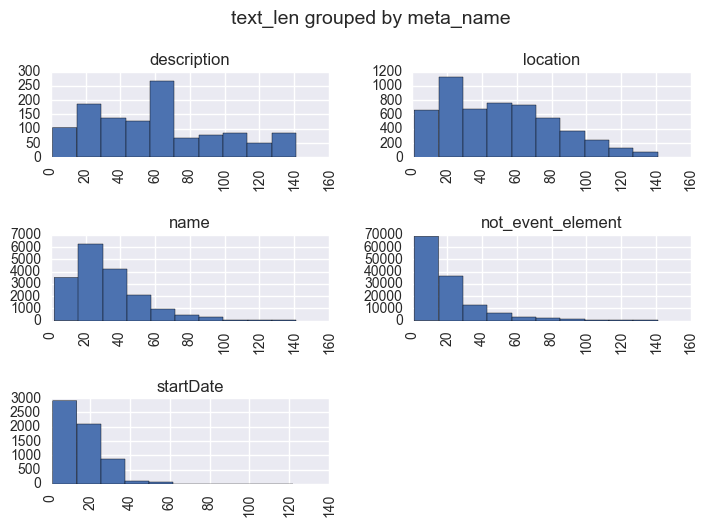
\includegraphics[width=1.0\textwidth]{figures07/distrTextByMeta}
\caption{Raw data-cleaning workflow}
\label{fig:distrTextByMeta}
\end{center}
\end{figure}

\begin{figure}[h]
\begin{center}
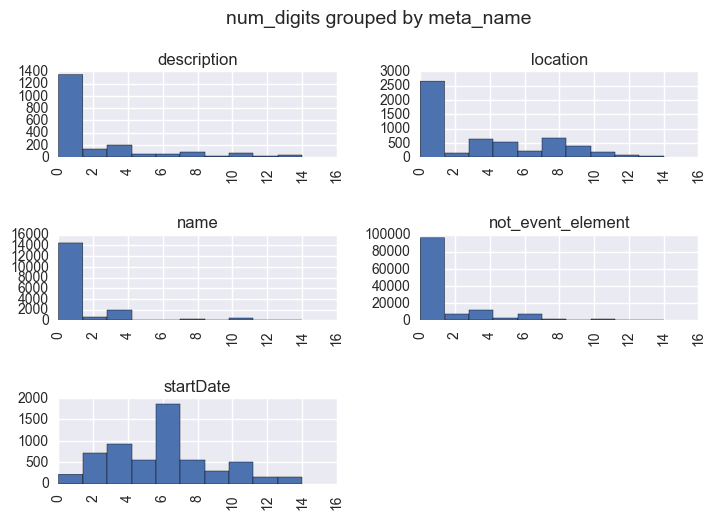
\includegraphics[width=1.0\textwidth]{figures07/distrDigitsByMeta}
\caption{Raw data-cleaning workflow}
\label{fig:distrDigitsByMeta}
\end{center}
\end{figure}


\subsection{Coordinates features}

After we extracted new features we got the following fileds in a dataset: {table:featurelist}.

\begin{table}[h]
\begin{center}
{\renewcommand{\arraystretch}{1.2}
\begin{tabular}{| p{6cm} | p{6cm} |}
\hline
\textbf{DOM}   &   \textbf{CSS}\\
\hline
URL of the page    &    Color (three chanells)\\
Meta name (name, startDate, description, location, no\_event)    &    Text alignment (center, left, right, etc)    \\
Text of the web element    &    Property of the block view    \\
HTML tag    &    The level font weight    \\
Number of siblings in a DOM tree    &    Padding    \\
Number of childs in a DOM tree    &    Font family (Verdana, Arial, etc)    \\
    &    Font size \\
    &    The language of the page \\
    
    &    \textit{+ 270 other CSS features} \\
\hline
\textbf{Visual}   &   \textbf{Textual}  \\
\hline
X and Y coordinate on the rendered picture    &    Length of the text inside the block    \\
X and Y coordinate of the center of a visual block    &    Number of punctuation marks in text    \\
Visual block height     &    Number of digits in text    \\
Visual block width        &    Number of digits/text length    \\
Height in a browser     &    Number of upper case letters    \\
Width in a browser     &    Number of whitespaces    \\

     &    \textit{+ tf-idf matrix}    \\
\hline
\end{tabular}}
\caption{List of main extracted features after feature engineering}
\label{table:featurelist}
\end{center}
\end{table}    
    
    



\section{Description of the dataset}
As a clean final dataset we have a table of 168K rows and 32 columns. Let's look at the main properties of the dataset: 

\begin{itemize}
    \item It contains 33K unique URLs, and  4000 domain names. 
    \item There are in average 45 URLs per one domain name. 
    \item We have 137K rows related to a random elements on the webpage, 18K for a event's name, 6K for a start date, 6K for location, and 2K for description. In sum, 32K rows containing features of event components. 
    \item There a in average 1.8 event components out of 4 on a webpage. 
    \item There are the most popular combinations of event components fro one URL. 
    \begin{itemize}
        \item \textit{name} 8335
        \item \textit{location, name} 2863 
        \item \textit{name, startDate} 2522 
        \item \textit{location, name, startDate} 1735
    \end{itemize}
    Top 10 list of combinations you may find in table \nameref{table:top10comb}.
    \item We have 30 numeric features and 4 textual. Additionaly, we will include \textit{idf-idf} matrix later.
    \item We replaced outliers of numerical features with the NaN. We fill the missing values with the corresponding average values.  
    \item 
\end{itemize}


\begin{table}
\begin{center}
{\renewcommand{\arraystretch}{1.5}
\begin{tabular}{| p{8cm} | p{2cm}|}
\hline
\textbf{Combination}	&	\textbf{Count}\\
\hline
['name']	&	8335\\
\hline
['location', 'name']	&	2863\\
\hline
['name', 'startDate']	&	2522\\
\hline
['location', 'name', 'startDate']	&	1735\\
\hline
['description', 'name']	&	730\\
\hline
['description', 'name', 'startDate']	&	548\\
\hline
['description', 'location', 'name']	&	485\\
\hline
['description', 'location', 'name', 'startDate']	&	293\\
\hline
['name', 'startDate', 'startDate']	&	246\\
\hline
['location', 'name', 'startDate', 'startDate']	&	125\\
\hline
\end{tabular}}
\caption{Top 10 combinations of event component for one URL}
\label{table:top10comb}
\end{center}
\end{table}	

\section{Analysis of features}

\begin{table}
\begin{center}
{\renewcommand{\arraystretch}{1.5}
\begin{tabular}{| p{0.8cm} | p{2cm}|  p{2cm}|  p{2.3cm}|  p{2.3cm}|  p{2.4cm}|}
\hline
\textbf{stat}	&	\textbf{color\_r}	&	\textbf{font\_size}	&	\textbf{font\_weight}	&	\textbf{digits\_share}	&	\textbf{block\_height}\\
\hline
count	&	167872.0	&	167872.0	&	167872.0	&	167872.0	&	167872.0\\
\hline
mean	&	76.396201	&	14.69536	&	455.510746	&	0.112503	&	26.359833\\
\hline
std	&	84.989934	&	4.15742	&	129.067880	&	0.225118	&	18.612600\\
\hline
min	&	0.0	&	0.0	&	100.0	&	0.0	&	0.0\\
\hline
25\%	&	4.0	&	13.0	&	400.0	&	0.0	&	16.0\\
\hline
50\%	&	51.0	&	14.0	&	400.0	&	0.0	&	19.0\\
\hline
75\%	&	125.0	&	16.0	&	400.0	&	0.117021	&	31.0\\
\hline
max	&	255.0	&	100.0	&	900.0	&	1.0	&	194.0\\
\hline
\end{tabular}}
\caption{Summary statistics for some numerical features}
\label{table:sumstatnum}
\end{center}
\end{table}	
















\section{Visualization}



